\scanpage{94}
\[
\unsure{h|\ell}_0\ h_1\ h_2\longrightarrow
\begin{aligned}
&\deleted{\unsure{h_1h_0h_1^{-1}}h_0^{\unsure{1|0}}h_1}\\
&\deleted{h_0^{\unsure{\alpha_0}}h_1}
\end{aligned}
\]
\figure{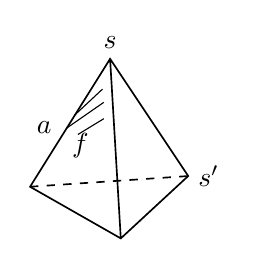
\begin{tikzpicture}[line width=.6pt,scale=.8]
\draw (-1.27,.02)--(0,2.05)--(1.24,.19)--(.17,-.8)--cycle (0,2.05)--(.17,-.8);
\draw[dashed] (-1.27,.02)--(1.24,.19);
\draw[thin] (-.57,1.15)--(-.12,1.57) (-.69,.95)--(-.1,1.36) (-.51,.85)--(-.1,1.1);
\node[above] at (0,2.05) {$s$}; \node[right] at (1.24,.19) {$s'$}; \node[left] at (-.77,.96) {$a$}; \node at (-.47,.67) {$f$};
\end{tikzpicture}}
\[
\begin{aligned}
 &(\overset{3}{\rho_f},\overset{3}{\rho_s},\overset{2}{\rho_a}) &&\unsure{3_3|\mathfrak S_3}\\
 &\rho_{s'}=\rho_f^{-1}\rho_s &&
 \begin{array}{l|l}
 \rho_{-1,1.}&(3,3,2)\longleftrightarrow(3,3,3)^-\\
 \rho_{1,-1.}&\deleted{\unsure{(3,3,2)}}\longleftarrow
 \end{array}\\
 &\rho_f\ \underset{\substack{\rotatebox{90}{$=$}\\\rho_{f'}}}{\rho_s^{-1}}
 &&\rho_{.\deleted{\unsure{-1}}-1,1}\\
 &\deleted{\rho_f}\quad\underset{\substack{\rotatebox{90}{$=$}\\\rho_{f'}}}{\rho_s^{-1}}\quad
 \underset{\substack{\rotatebox{90}{$=$}\\\rho_{a'}}}{\rho_a}
 &&\left\{\begin{array}{cc}(3,3,2)^+&\unsure{3.}\quad(3,3,2)^-\\
 (3,3,3)^+&(3,3,3)^-\end{array}\right.
\end{aligned}
\]
${\unsure{G|\mathfrak S|\mathcal S}}_3\cdot$\qquad opère sur \unsure{un|nos} ens à $8$ él.
\[
\begin{aligned}
\left.\begin{aligned}
 (3,3,2)^+ &\underset{\deleted{\rho_{-1,1,.}}}{\longleftrightarrow}(3,3,3)^+\\
 (3,3,2)^- &\longleftrightarrow(3,3,3)^-
\end{aligned}\right|&\ \rho_{-1,1,.}\\
\left.\begin{aligned}
 (3,3,2)\\ 3,3,2
\end{aligned}\right|&\ \rho_{1,-1,.}
\end{aligned}
\qquad
\tau_{01}\rho_{\alpha,1.}\tau_{01}^{-1}=\rho_{1,\alpha.}
\]
\[
\begin{aligned}
 &G_3*\mathbb Z/2\mathbb Z\\
 &\quad\unsure{\mathord{/}\ \rotatebox{90}{$\simeq$}|\wr\mathrel{\Vert}}\\
 &\deleted{\unsure{\mathbb Z}}\ G_3\cdot{\mathbb Z}_{/2\mathbb Z}^{(*G_3)}\\
 &\qquad\qquad\rho^\sigma(\varepsilon)
\end{aligned}
\]
\[
\begin{aligned}
&\unsure{\rho^{?}|\deleted{\rho_{\cdot}}}\qquad\\
&\rho_1^{\{01\}}((\varepsilon,1))\\
&\rho^{\{0,1\}}(\varepsilon,\varepsilon')\\
&\deleted{\rho_\sigma\quad\rho}
\end{aligned}
\qquad
\begin{aligned}
 &\rho(\varepsilon)\ \text{commute à}\ \rho^\sigma(\varepsilon),\\
 &\text{si }\sigma\text{ est une \inserted{de 2} transposition}\\
 &\deleted{\text{qui \unsure{change} }0.}\quad\inserted{\pi_{01},\pi_{02}}
\end{aligned}
\]
\[
\begin{aligned}
 &\varepsilon_\sigma\qquad(\sigma\in G_3)\\
 &\varepsilon_1=\rho^{\{01\}}\deleted{(\unsure{+1|1},1}(-1,1)=\rho_{-1,1.}\\
 &\pi\varepsilon_{\unsure{1|7}}\pi^{-1}=\rho_{1,-1.}\qquad\pi=\pi_{01}
\end{aligned}
\]
% archive sheet number: 93
